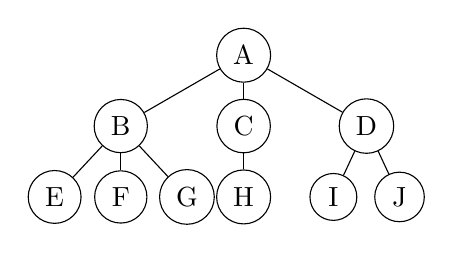
\begin{tikzpicture}[scale=0.6]
  \tikzstyle{every node}=[draw]
  \node [circle] at (0,0) {\tf A}[sibling distance=2.6cm] 
  child { node[circle]{\tf B}[sibling distance=1.4cm]
    child {node[circle]{\tf E}}
    child {node[circle]{\tf F}}
    child {node[circle]{\tf G}}      
  }    
  child { node[circle]{\tf C}
    child {node[circle]{\tf H}
    }			
  }	
  child { node[circle]{\tf D}[sibling distance=1.4cm]
    child {node[circle]{\tf I}}
    child {node[circle]{\tf J}}
  };  
\end{tikzpicture}
